\section*{Abstract}
Earth Observation by means of remote sensing imagery and gridded environmental data opens tremendous opportunities for systematic capture, quantification and interpretation of plant - environment interactions through space and time. The acquisition, maintenance and processing of these data sources, however, requires a unified software framework for efficient and scalable integrated spatio-temporal analysis taking away the burden of data and file handling from the user. Existing software products either cover only parts of these requirements, exhibit a high degree of complexity, or are closed-source, which limits reproducibility of research. With the open-source Python library EOdal (Earth Observation Data Analysis Library) we propose a novel software that enables the development of fully reproducible spatial data science chains through the strict use of open-source developments.
Thanks to its modular design, EOdal enables advanced data warehousing especially for remote sensing data, sophisticated spatio-temporal analysis and intersection of different data sources, as well as nearly unlimited expandability through application programming interfaces (APIs).

\section{Introduction}
Images from Earth Observation (EO) satellites and in-situ observations are of great importance for ecophysiological \citep{caparros-santiago_land_2021} and agroecological research \citep{karthikeyan_review_2020}. Such data can be used to determine plant traits and allow mapping of plant growing conditions for larger areas using standardized methods \citep{weiss_remote_2020}. Open-access, high-resolution satellite data such as from the European Space Agencies' Sentinel-2 (S2) mission can resolve field heterogeneity and provide site-specific farming measures operationally. Examples include yield estimates \citep{marshall_optimizing_2018,perich_pixel-based_2022}, extraction of phenological metrics \citep{duarte_qphenometrics_2018}, variable irrigation rates \citep{barker_evaluation_2018} and site-specific fertilization scheduling \citep{mittermayer_analysis_2022}. Remotely sensed plant traits and their dynamic development over time  can further be augmented with environmental covariates such as climate, soil and terrain data, as well as information about farm management to perform integrated analysis on material and energy fluxes across spatio-temporal scales \citep{asam_relationship_2018}.

However, accessing, managing and analyzing EO data is complex and often requires solid knowledge of geographic information science and coding to properly handle large spatial data sets. We base this finding on an exhaustive review of existing software tools. For example, the philosophy of the OpenDateCube \footnote{\url{https://www.opendatacube.org/}} initiative is about integrated analysis of EO data using standardized interfaces. Installing the software, however, is complex as setting up a database instance is required. The Framework for Operational Radiometric Correction for Environmental monitoring (FORCE) \citep{frantz_forcelandsat_2019} is primarily designed for the creation of Analysis-Ready-Data (ARD) but does not provide interfaces for data analysis workflows. Analysis workflows using standardized interfaces are the main subject of the openEO\footnote{\url{https://openeo.org/}} project. openEO, however, focuses on cloud environments. Thus, data sets that are not available on externally operated web platforms are currently excluded. This applies particularly to (experimental) research data sets. Researchers therefore often spend a significant amount of time getting the data into an analysis-ready format. Based on the analysis of more than 3000 productive machine learning pipelines at Google, \citet{xin_production_2021} identified great potential for optimization in the area of data management and pre-processing, which also appears to be true in the EO area.

For these reasons, we developed the Earth Observation Data Analysis Library (EOdal) as an open-source Python (3.8+) package designed to make EO data analysis tools available to researchers without the need for in-depth knowledge about geoinformation science, coding and remote sensing data handling. A key aspect of EOdal is the ability to apply spatial data science methods to data from different sources within a unified framework based on open-source tools. We also intend to provide researchers with an alternative to proprietary software solutions such as the widely used Google Earth Engine \citep{gorelick_google_2017}.

The functionality and structure of EOdal is explained in Section \ref{sec:package_struc} of this paper. In Section \ref{sec:reprod_example}, we present a reproducible use case based on an agricultural research question followed by a discussion in Section \ref{sec:conclusions}.

\section{Description of EOdal}
\label{sec:package_struc}
EOdal consists of three layers as shown in Figure \ref{fig:overview}. The layers are organized in a triangle to emphasize their inter-dependencies. The core layer (Figure \ref{fig:overview}, top) provides the Python classes required to perform I/O operations to read and write geo-spatial data sets in a generic way. It is also the basis for data warehousing, i.e., the storage of metadata. Class inheritance extends its capabilities to specific EO sensors such as S2 Multispectral Imager (e.g., for convenient reading of data organized in the Satellite Archive for Europe structure). (Pre-)processing of these datasets is accomplished in the processing layer (Figure \ref{fig:overview}, lower right). Processing steps such as spatial reprojection are often a necessity to combine different datasets for analysis. The analysis layer (Figure \ref{fig:overview}, lower left) enables automatized, reproducible EO data management and is the backbone for data-driven analysis of geo-spatial data sets and their spatio-temporal intersection.

Deployment of EOdal is independent of an Operating System. Furthermore, EOdal can be used on local premises (e.g. for processing research datasets) but also in cloud environments for fast access to large, freely accessible data such as the global S2 or Landsat archive. To enable fast and scalable deployment required for large-scale analysis tasks EOdal can be installed into containerized environments (Docker containers).

\subsection{Core Layer}
The data model of the core layer (Figure \ref{fig:overview} top) follows the object-oriented programming paradigm and includes different classes. There are three classes in the EOdal core layer: Bands, RasterCollections and derived (inherited) sensor-specific classes. The Band class represents the base class. In simple terms, a Band refers to a two-dimensional array referenced in a geo-spatial coordinate reference system. A RasterCollection is a collection of zero to $n$ Band objects, which can exist in different spatial reference systems, grid cell sizes (pixel sizes) and spatial extents. Band objects in a collection are identified by names (e.g., "blue", Figure \ref{fig:overview} top right) instead of numeric indices. Bands and RasterCollections can be created from any geo-referenced raster data set understood by Geospatial Data Abstraction Library (GDAL, e.g., GeoTiff), vector features (e.g. Shapefile, GeoJSON), and from numerical arrays (Python libraries, e.g. NumPy, Zarr). Sensor-specific RasterCollections include all the functionalities and attributes of the RasterCollection class, but are tailored to the requirements and capabilities of specific imaging sensors such as, for example, S2, or Landsat. The inheritance-based software design allows the introduction of further sensors and makes the core layer extensible also with regard to upcoming future EO platforms such as the hyperspectral Copernicus expansion mission CHIME\footnote{\url{https://www.esa.int/Applications/Observing_the_Earth/Copernicus/Going_hyperspectral_for_CHIME}} and beyond.

A further central element of the core layer is the collection of metadata in a spatio-temporal catalog  allowing the filtering of records by data source, time period, and geographic region of interest (ROI). EOdal supports Spatio-Temporal Asset Catalogs (STAC), which are available in many cloud environments that provide geo-spatial (satellite) data, such as Microsoft Azures Planetary Computer\footnote{\url{https://planetarycomputer.microsoft.com/}}, Amazon Web Services (AWS) Earth\footnote{\url{https://aws.amazon.com/de/earth/}} and the Copernicus Data and Information Access Services (DIAS). For local deployment, EOdal offers the possibility to store metadata in a PostgreSQL database with the spatial PostGIS extension.

In terms of spatial data models and standards, EOdal supports area (polygons and multi-polygons) as well as point features following the general feature model defined in the ISO 19109 standard \citep{iso_iso_2015}. This allows point-based in-situ observations, for example from weather stations or ground sensors, to be intersected with EO data and auxiliary data sources such as Digital Elevation Models (see Section \ref{sec:reprod_example}).

\subsection{Processing Layer}
\label{subsec:processing-layer}
The processing layer (Figure \ref{fig:overview}, lower right) provides functionalities for EO data preparation and (pre-)processing. Data preparation is usually necessary to enable the merging datasets from different sensors and platforms. This includes image manipulation methods such as spatial resampling and reprojection from one coordinate system into another or masking operations to mask out bad quality observations or land cover classes.

\subsection{Analysis Layer}
The analysis layer (Figure \ref{fig:overview}, bottom) is used for the analysis of data from EO satellites and environmental covariates such as meteorological, terrain, soil and land use data. It builds upon the core layer to query and access different data sources and the processing layer to prepare the data analysis-ready. The underlying complex data management such as the merging of data from satellite tiles and filling of no-data values is hidden from the user in the processing layer (see Section \ref{subsec:processing-layer}).

EOdal provides interfaces to widely-used open-source Python libraries (e.g., geopandas, numpy, xarray). This allows users to integrate their own EO processing workflows and modules (c.f. section \ref{subsec:supplementary-modules}) to e.g. estimate biochemical, structural or integrated traits such as chlorophyll, leaf area index, yield or land surface phenology (Figure \ref{fig:overview}, lower left). 

\subsection{Applications of EOdal}
\label{subsec:supplementary-modules}
EOdal has already been used for studies in agroecological research. \citet{perich_pixel-based_2022} used EOdal for pixel-based prediction of crop yield using S2 time series.  In \citet{graf_propagating_2022}, EOdal is used to propagate radiometric uncertainty from S2 reflectance factors to phenological metrics. Moreover, EOdal drives the EO platform at the Swiss Federal Center of Excellence for Agricultural Research, Agroscope, underpinning its relevance within an operational and governmental environment\footnote{\url{http://www.eoa-team.net/}}.

\begin{figure}[H]
    \centering
    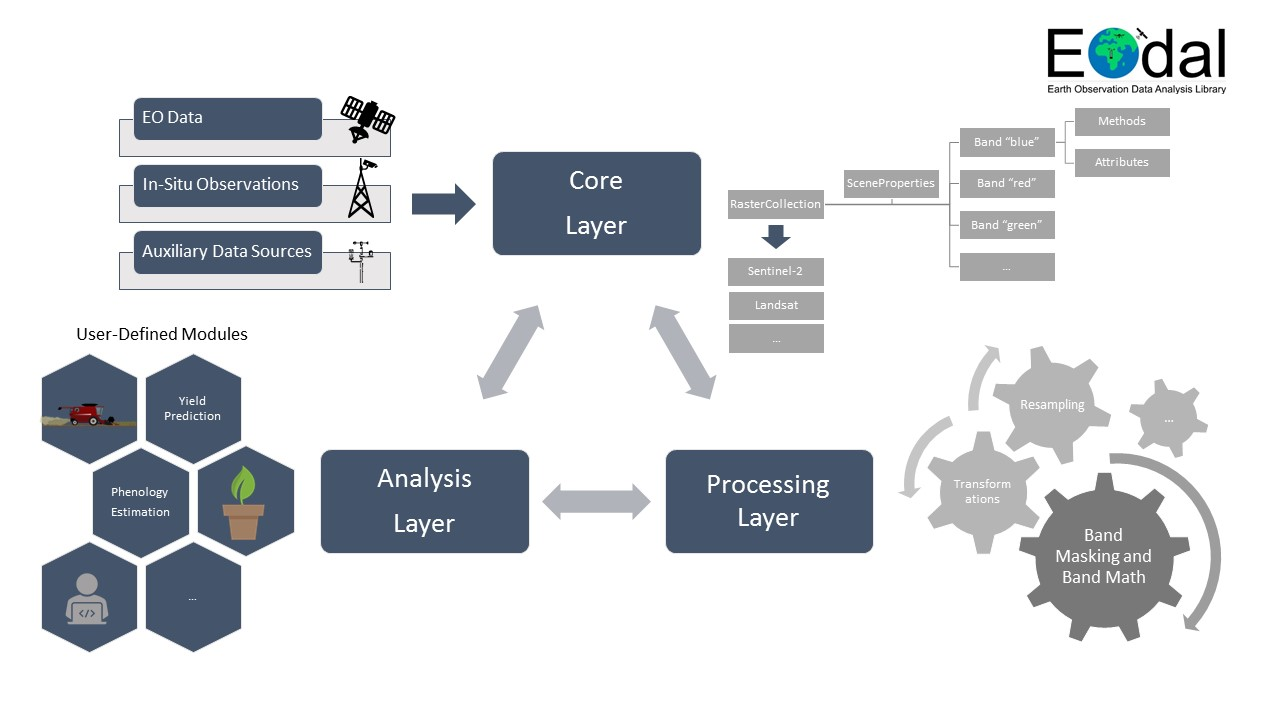
\includegraphics[width=\textwidth]{EOdal_layers.jpg}
    \caption{Overview of EOdal and its three layers: The core layer (top) handles different input data sources in a standardized way. The analysis layer (bottom left) builds upon the core and the processing layer (bottom right) for data maintenance, querying, intersection and integration into user-defined data science pipelines.}
    \label{fig:overview}
\end{figure}

\section{Usage Example: Interpreting In-Field Growth Heterogeneity Through Time with Topographic and Meteorological Data}
\label{sec:reprod_example}
We illustrate here the potential of EOdal for integrated spatio-temporal analysis over an example ROI from western Switzerland near Lake Neuchâtel ($46.98^\circ N$, $7.07^\circ E$). All results were produced by a single Jupyter notebook (\url{https://doi.org/10.1016/j.compag.2022.107487}) running EOdal v0.0.1 on Microsoft Planetary Computer. Due to large-scale land subsidence, the entire region - a former peat land - is subject to increased flood risk \citep{egli_landschaftsdynamik_2020}. An agricultural parcel (12 ha) was affected by flooding during heavy rainfall (360 mm within 30 days) between mid-June and July 2021, causing flood damage to the previously homogeneous green canopy. Figure \ref{fig:s2-fig} shows S2 derived false-color infra-red images of the parcel in 2021 before the flood (reddish tones in Figure \ref{fig:s2-fig}a). In the spring 2022, differences in canopy greenness of the emerging winter wheat are evident (Figure \ref{fig:s2-fig}b and c). Darker areas, which indicate lower soil cover, can be discerned in the otherwise red-colored canopy. The spatial pattern within the field corresponds to the patterns within the DEM (Figure \ref{fig:s2-fig}e) and reveals that parts with lower elevation values were more impacted by flooding than the rest of the field. Extraction of the Modified Soil Adjusted Vegetation Index (MSAVI, \cite{qi_modified_1994}) time series from two selected S2 pixels (Figure \ref{fig:s2-fig}d) allows to evaluate the impact of the flood in 2021 on the growth dynamic in 2022 and confirms the findings from the false-color S2 images.
As additional usage example, the growth pattern of a field is investigated in relation to meteorological data, often used to validate and calibrate ecophysiological growth models. In this case (Figure \ref{fig:s2-fig}f), the cumulative growing degree days (in °C) and cumulative daily rainfall amount (in mm) were derived from a nearby weather station (Ins) operated by the Swiss Federal Office of Meteorology and Climatology (MeteoSwiss) calculated from November \nth{1} 2021.

\begin{figure}[H]
    \centering
    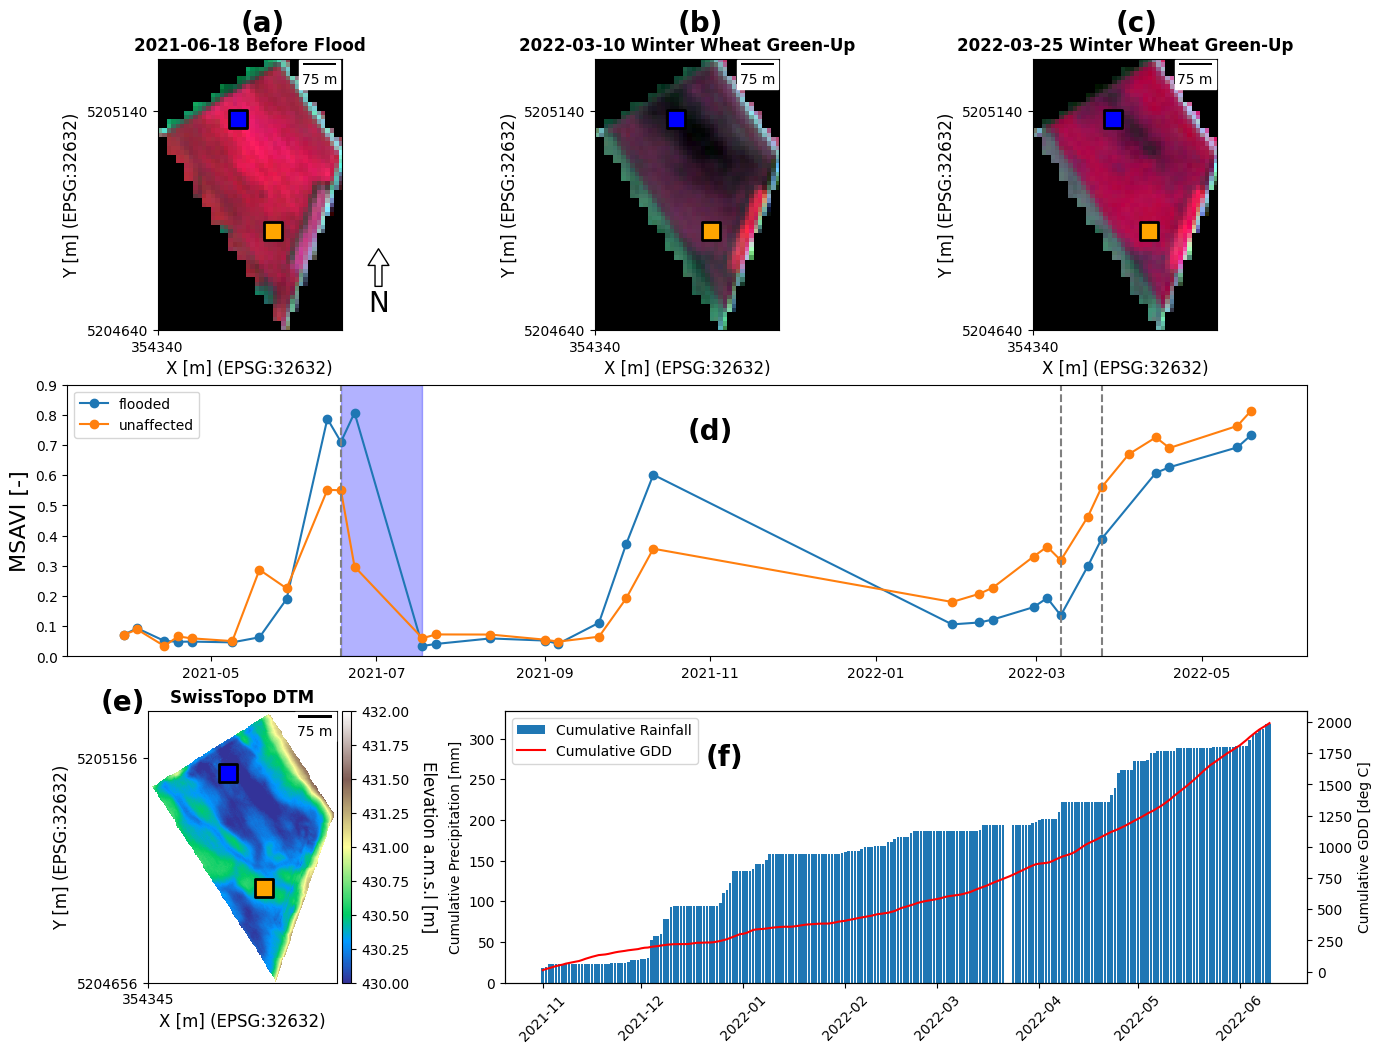
\includegraphics[width=\textwidth]{S2_Flood_Crop_Growth_Example.png}
    \caption{Result of a single Jupyter notebook run using EOdal (v0.0.1) on Microsoft Planetary Computer. S2 false-color infra-red composite of the field parcel before the heavy rainfall events in June and July 2021 (a) and spatial heterogeneity in winter wheat green-up during spring 2022 (b-c). In addition, cumulative growing degree days (GDD) and daily precipitation sums derived from a nearby weather station are shown (f). The extent of the flood in 2021 - evident as darker areas in (b-c) - corresponds to a depression visible in the Digital Elevation Model (e). The flood affected plant growing conditions in spring 2022 as shown in the MSAVI time series (d) of a 'flooded' pixel (blue) and a pixel that was little affected by the floods in 2021 (orange). The dashed lines in (d) correspond to the timing of (a), (b) and (c), respectively, whereas the blue rectangle in (d) indicates the approximate timing of the flooding in 2021.}
    \label{fig:s2-fig}
\end{figure}

\section{Discussion and Conclusion}
\label{sec:conclusions}
%\chapter{General discussion}
\label{chap:general-discussion}

The aim of this chapter is to bring together the different aspects of the research carried out (Chapters \ref{chap:eodal}-\ref{chap:drc}) within the framework of a landscape-scale prototype and to discuss its applications, limitations and possible further research questions. However, the scientific discussion of the individual research chapters is not repeated here. Please refer to the relevant discussion subsections in the previous chapters.

\section{A prototype for landscape-scale phenotyping}
Figure \ref{fig:oa-disc-prototype} shows a sketch of how the individual research components can be transferred to a landscape level prototype to quantify winter wheat growth and development.

The main data sources for the prototype are environmental covariates, mainly air temperature, and high resolution optical satellite imagery from the \gls{S2} mission. The necessary calibration of the prototype is mainly based on field phenotyping data, which encode the relationships between development and growth (see chapter \ref{chap:insights}) and establish the relationship between plant growth and environmental conditions (chapter \ref{chap:drc}). These calibration data thus represent the physiological and phenological knowledge of G $\times$ E interactions in crops in general and wheat in particular.

Using the calibration and the two data sources, the functionality of the prototype can now be demonstrated in three steps.

\paragraph{Step 1 -- Timing and duration of key phenological stages}
The first step is to determine the timing of key phenological development stages as described in Chapters \ref{chap:phemology} and \ref{chap:insights}. This is important to determine the onset and duration of the \gls{SE} period, which is the focus of attention due to its importance in grain yield formation, as explained in Chapter \ref{chap:introduction}. The phenology model uses only weather data and has a relatively coarse spatial resolution (km scale) due to the relatively coarse resolution of most meteorological data products at the landscape scale. The timing extracted from the phenology model will therefore limit the period over which satellite data should be considered.

\paragraph{Step 2 -- Trait retrieval from satellite imagery}
Once the relevant time period has been extracted, satellite data are searched and converted to \gls{GLAI} using physiological and phenological priors from field phenotyping as described in Chapter \ref{chap:insights} using RTM inversion and the software \gls{EOdal} (Chapter \ref{chap:eodal}). Thus, at $n$ time points, where $n$ is the number of \gls{S2} scenes, \gls{GLAI} estimates are available at 10 $\times$ 10 m spatial resolution. This allows spatial detail to be resolved, e.g. on within-field heterogeneity, which is not available from the temperature data. The \gls{GLAI} estimates based on the \gls{S2} data are thus snapshots of the apparent growth conditions.

\paragraph{Step 3 -- Reconstruction of growth}
Using the \gls{S2} \gls{GLAI} observations and the air temperature data, the growth dynamics in the \gls{SE} period can be modelled in hourly or daily resolution in a final step, as described in Chapter \ref{chap:drc} using \gls{DRC}s. In this way, the high temporal resolution of the temperature data is combined with the spatial detail of the \gls{S2} \gls{GLAI} observations. Here, not only the physiological knowledge from the field phenotyping is encoded, but also the uncertainty propagation carried out in Chapter \ref{chap:uncertainty} is used to model growth and development during the \gls{SE} period.

\begin{figure}[H]
    \centering
    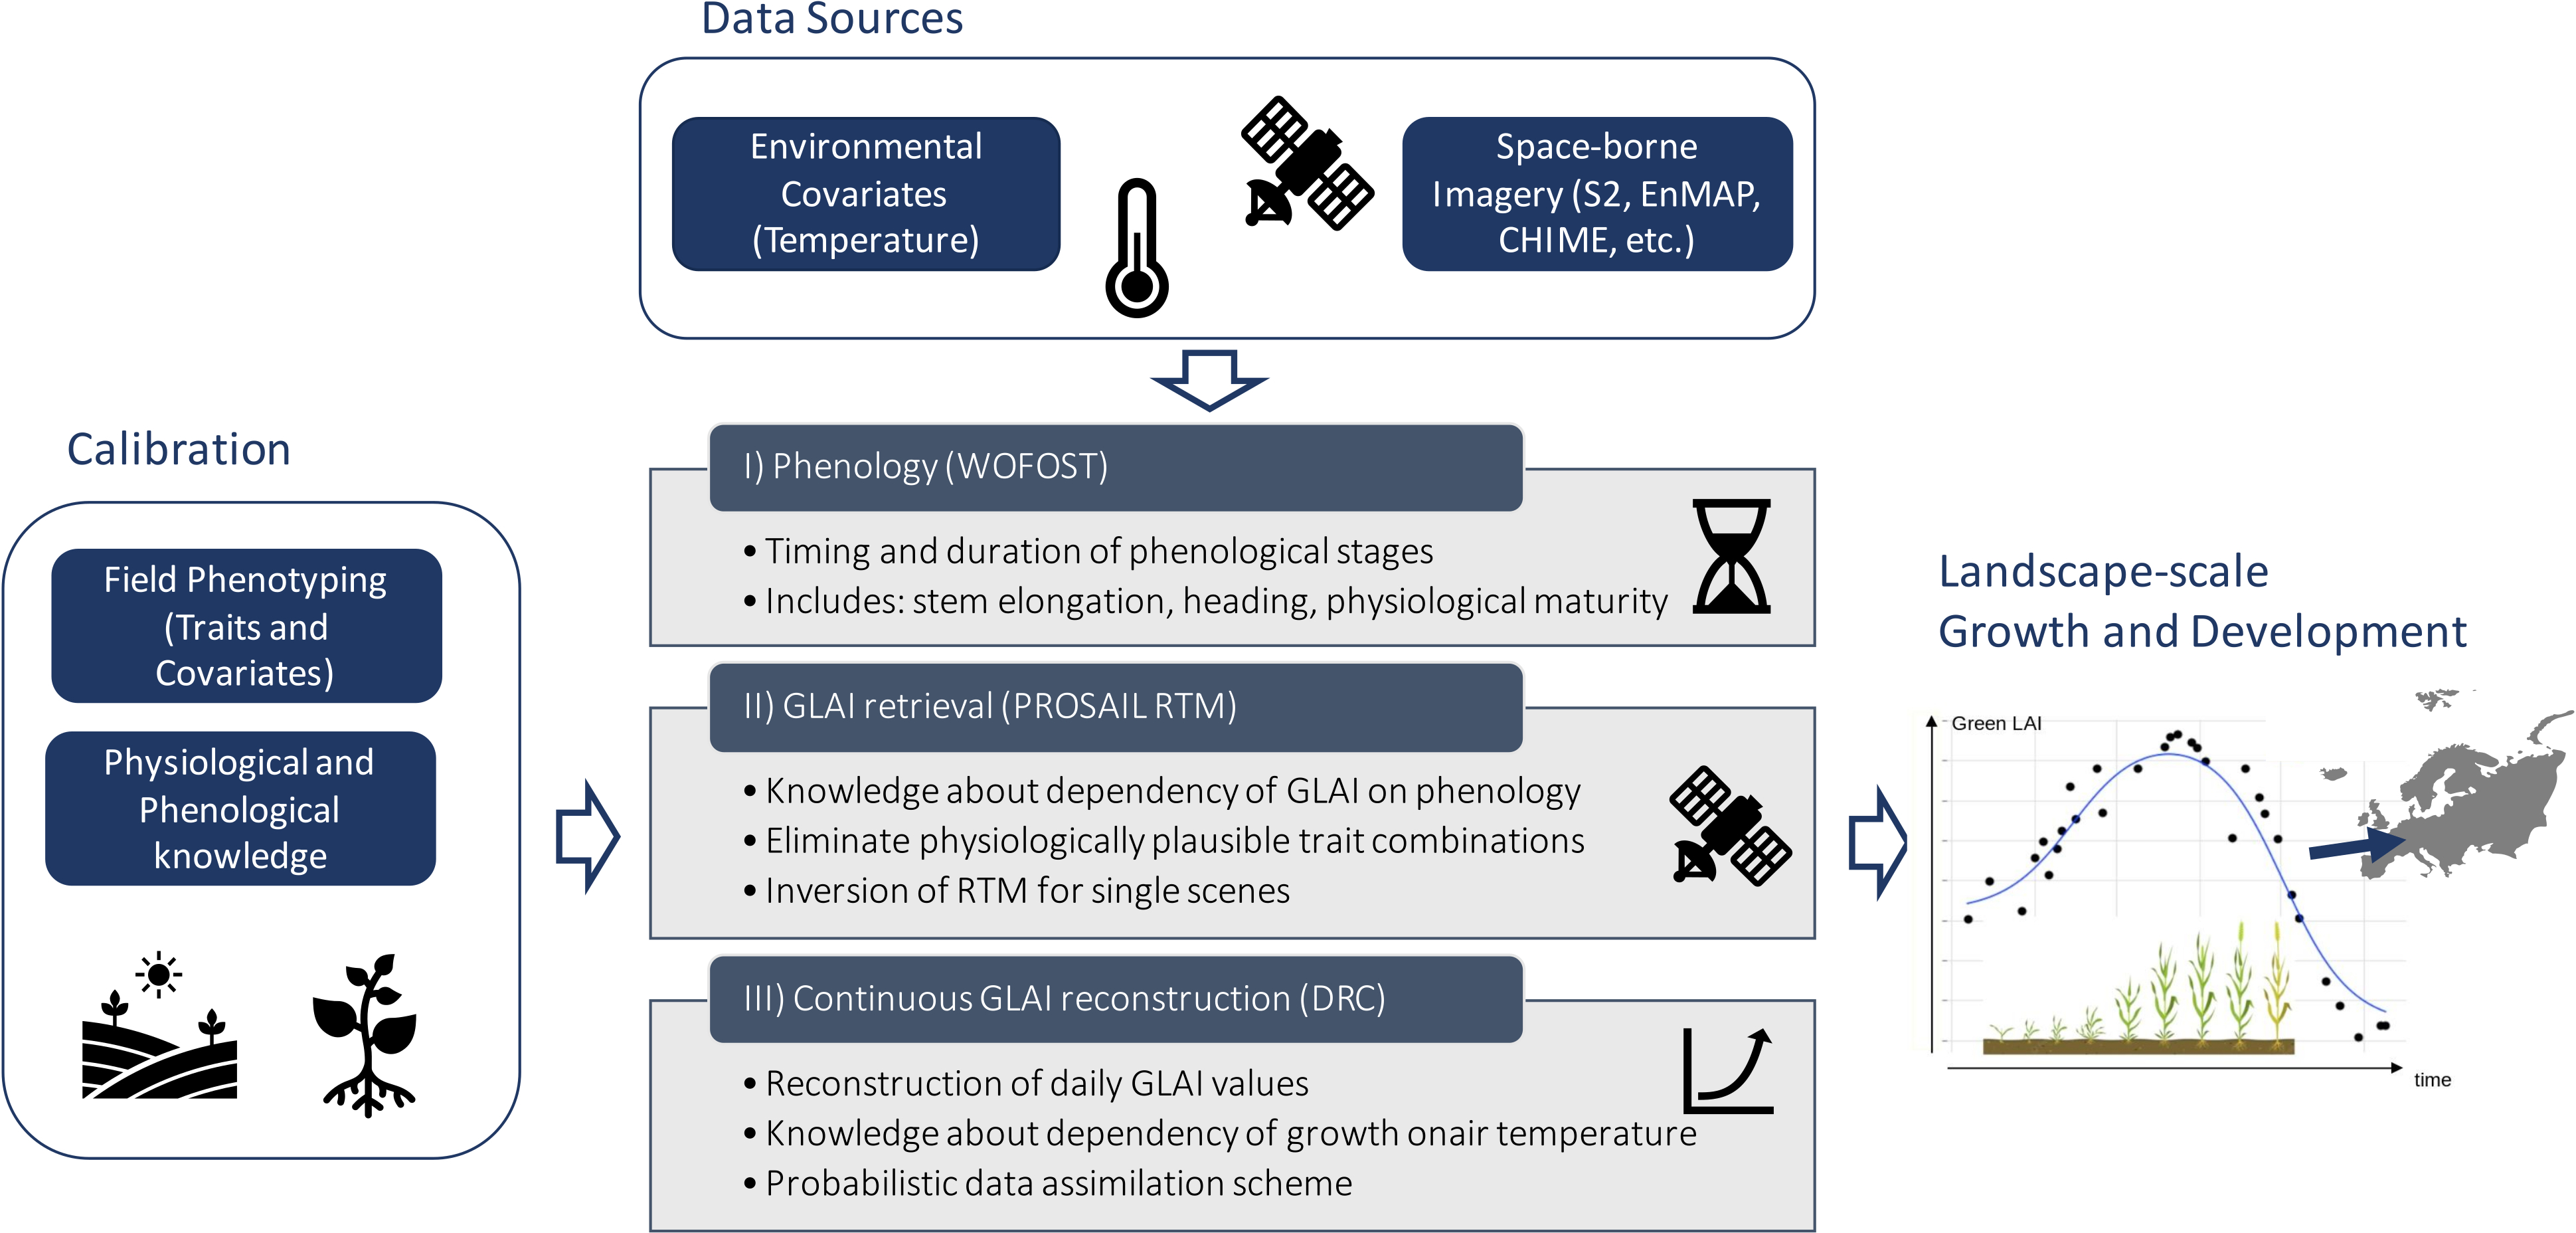
\includegraphics[width=\textwidth]{07-Discussion/img/prototype.jpg}
    \caption{The proposed prototype for landscape scale phenotyping of winter wheat growth and development as a key outcome of this thesis.}
    \label{fig:oa-disc-prototype}
\end{figure}

The prototype composed of these components thus allows the quantification of winter wheat growth and development at the landscape scale, for example in the Swiss Mittelland, with a spatial resolution of up to 10 m and a temporal resolution of up to one hour. Furthermore, by combining satellite, meteorological and in-situ data, the prototype can be considered as a true \gls{EO} system. At the same time, the quantification of growth through \gls{GLAI} values and development through phenological stages means that the prototype is also a phenotyping system. Overall, the prototype presented is in line with multilateral incentives such as \gls{GEOCLAM} that aim to provide traceable, actionable insights to stakeholders in agriculture \citep{whitcraft_no_2019}. As the prototype relies on open satellite and, at least in most cases, readily available temperature data and rather simple but physiologically meaningful models, it appears well suited for further operationalisation and near-realtime deployment.

\section{Answers to research questions}
With the prototype (Figure \ref{fig:oa-disc-prototype}) the three research questions outlined in section \ref{sec:intro-obj-rj} can be addressed.

\subsection{How can field phenotyping and spaceborne remote sensing data be combined to allow up-scaling of physiological knowledge from field phenotyping to the landscape-scale?}
This thesis has identified two ways of combining field phenotyping and spaceborne remote sensing data. The first way is to use field phenotyping data as prior knowledge to constrain \gls{RTM} simulations as shown in chapter \ref{chap:insights}, and to fill temporal gaps and remove outliers using \gls{DRC}s to reconstruct hourly or daily \gls{GLAI} trajectories from single \gls{S2} observations (Chapter \ref{chap:drc}). While the first way directly addresses the workflow of remote sensing retrieval and time series reconstruction, the second way is about using field phenotyping data to parameterise phenological models (Chapter \ref{chap:phemology}), which in turn are used to select relevant satellite imagery and quantify the timing of key developmental stages such as the end of heading. It is thus a more indirect way of incorporating field phenotyping data into an \gls{EO} approach. As a result, both pathways allow knowledge and concepts to be scaled up from field phenotyping to the landscape scale.

\subsection{Can a landscape-scale phenotyping approach provide accurate, physiologically based and traceable insights into winter wheat growth and development?}
The quantification of uncertainties (see Chapter \ref{chap:uncertainty}) fulfils the requirement for traceability (Section \ref{sec:intro-obj-rj}). The integration of prior knowledge from field phenotyping into the \gls{GLAI} retrieval process in step 2, as well as into the parameterisation of \gls{DRC}s in step 3, fulfils the requirement for physiological plausibility (see also the individual scientific discussions in Sections \ref{sec:insights_discussion} and \ref{sec:drc_discussion}). The accuracy of the methodology has been demonstrated using multi-year, independent in-situ data for phenological development (RMSE for heading date: 2 days, Chapter \ref{chap:phemology}) and GLAI (smallest relative error: 13\%, Chapter \ref{chap:drc}). This research question can therefore be answered in the affirmative.

\subsection{What are the potentials but also the limitations and challenges of such a landscape phenotyping approach?}

The prototype allows the study of G $\times$ E interactions that could not be fully addressed by small-scale field phenotyping experiments. These include effects of changes in soil properties or topography that are spatially continuous and affect plant growth and development through soil water availability, exposure to wind and sunlight, or nutrient availability. In addition, the \gls{GLAI} estimates can be converted to biomass \citep{aase_relationship_1978} and -- in perspective -- grain yield, which are arguably important agronomic traits for decision making and policy advice. Accurate modelling of these traits will therefore not only advance the science behind \gls{EO}-based applications for agriculture, but also help to meet the needs of a growing world population.


% lack of further calibration data
% lack of management data -> varieties (paper dario with share of varieties); sowing date lacking
% scalability: that's a core promise of RS but holds only true for the radiative properties; the translation into traits is more difficult!

\section{Open questions}
\subsection{Spatial or temporal detail?}

\subsection{What are the limiting factors?}
% we worked with temperature, only!
% the questions is: what are the limiting factors of growth and development
% do not forget about the management!

\section{Outlook}
% extend to senescence phase -> grain filling phase
% different crops -> other cereals but also pulses, etc.
% include different RS data sources (Planet, S1, etc.)
% methodology
The usage example shown in Figure \ref{fig:s2-fig} highlights how EOdal can be used to combine different environmental covariates with vegetation dynamics obtained from satellite time series to develop a holistic understanding of plant-environment interactions. This simple example shows how EOdal lowers the barriers of entry to EO analysis unlocking potential for data-based decision-making in agroecology. In addition, by using Docker and cloud infrastructure, the analysis can be extended to larger spatial and temporal scales. For the future we envision an ecosystem of user modules that build on EOdal, complement themselves and are developed and made freely available to the EO community. 

EOdal is in line with recent developments in agriculture that allow (technically inexperienced) users to run complex analyses: \citet{godara_agrimine_2022} developed a platform called "AgriMine". The platform enables spatio-temporal analysis of issues in Indian agriculture based on help-desk calls improving the Indian agricultural extension service. Improvements in variety testing were enabled by an online platform in China that makes processes more efficient and lines up with recent incentives in high-throughput phenotyping efforts \citep{pan_online_2022}. Similarly, EOdal can contribute to increased use of EO data in agriculture.

Although we focus on agriculture (section \ref{subsec:supplementary-modules}), EOdal is not limited to it. Rather, EOdal can be used in all disciplines that process EO data and require open, reproducible data analysis workflows. Thus, we expect EOdal to trigger further open-source developments, either through the release of additional Python packages that build on the existing functionalities, or through its integration into existing data processing frameworks. Ultimately, EOdal is intended to provide researchers with an alternative to proprietary software platforms while also easing the burden of data management for practitioners. For this reason EOdal is particularly well suitable for educational activities in the field of EO. This supports the transition to reproducible science, benefiting the EO community as a whole.

\section*{CRediT Authorship Contribution Statement}
Lukas Valentin Graf: Conceptualization, Software, Investigation, Visualization, Writing – original draft, Writing – review \& editing. Gregor Perich: Conceptualization, Software, Writing – original draft, Writing – review \& editing. Helge Aasen: Supervision, Writing – original draft, Writing – review \& editing.

\section*{Declaration of Competing Interest}
The authors declare that they have no known competing financial interests or personal relationships that could have appeared to influence the work reported in this paper.

%% create a non-numbered section for the Acknowledgements
\section*{Acknowledgements}
The authors thank Achim Walter from the Crop Science group at ETH for providing the IT infrastructure and in particular Norbert Kirchgessner for his support with data storage and implementation. Furthermore, we thank Alfred Burri for on-site support and contributions to the usage example and Fabio Oriani for valuable comments on the manuscript. The development of EOdal was conducted within the project `PhenomEn' funded by the Swiss Science Foundation (grant number IZCOZ0\_198091). GP acknowledges funding through the project `DeepField' of the Swiss Federal Office for Agriculture (BLW). 